% To familiarize yourself with this template, the body contains
% some examples of its use.  Look them over.  Then you can
% run LaTeX on this file.  After you have LaTeXed this file then
% you can look over the result either by printing it out with
% dvips or using xdvi.
%

\documentclass[twoside]{article}
%\usepackage{soul}
\usepackage{./lecnotes_macros}


\begin{document}
%FILL IN THE RIGHT INFO.
%\lecture{**LECTURE-NUMBER**}{**DATE**}{**LECTURERS**}{**SCRIBE**}
\lecture{6}{The Retracing Boomerang Attack}{Maria Francis and M. V. Panduranga Rao}{Gautam Singh}{26 March 2025}
%\footnotetext{These notes are partially based on those of Nigel Mansell.}

%All figures are to be placed in a separate folder named ``images''

% **** YOUR NOTES GO HERE:

\section{Introduction}

The retracting boomerang attack broke the record for 5-round AES when it was
published, bringing the attack complexity down to \(2^{16.5}\)
encryption/decryption operations. It uncovers a hidden relationship between
boomerang attacks and two other cryptanalysis techniques, namely the yoyo game
and mixture differentials.

\section{Preliminaries}

\subsection{Boomerang Attacks}

The working of a boomerang attack is shown in \autoref{fig:boomerang}. 

\begin{figure}[!ht]
    \centering
    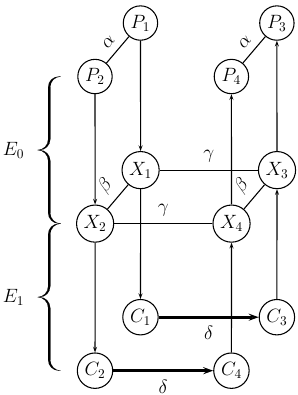
\includegraphics[width=0.3\columnwidth]{images/boomerang.png}
    \caption{The boomerang attack.}
    \label{fig:boomerang}
\end{figure}

Boomerang attacks typically split the encryption function as \(E = E_1 \circ
E_0\), with differential trails for each sub-cipher. Consider \(\alpha
\rightarrow \beta\) to be the differential characteristic in \(E_0\) with
probability \(p\) and \(\gamma \rightarrow \delta\) to be the differential
characteristic in \(E_1\) with probability \(q\). Then, one can build a
distinguisher that can distinguish the full cipher \(E\) from a truly random
permutation in \(\cO\brak{\brak{pq}^{-2}}\) plaintext pairs. This is shown in
\autoref{alg:boomerang-dist}.

\begin{algorithm}
    \caption{The Boomerang Attack Distinguisher}
    \label{alg:boomerang-dist}
    \begin{algorithmic}[1]
        \State Initialize a counter \(ctr \gets 0\). 
        \State Generate \(\brak{pq}^{-2}\) plaintext pairs \(\brak{P_1, P_2}\)
        such that \(P_1 \oplus P_2 = \alpha\).
        \ForAll {pairs \(\brak{P_1, P_2}\)}
            \State Ask for the encryption of \(\brak{P_1, P_2}\) to \(\brak{C_1,
            C_2}\).
            \State Compute \(C_3 = C_1 \oplus \delta\) and \(C_4 = C_2 \oplus 
            \delta\). \Comment{\(\delta\)-shift}
            \State Ask for the decryption of \(\brak{C_3, C_4}\) to \(\brak{P_3,
            P_4}\).
            \If {\(P_3 \oplus P_4 = \alpha\)}
                \State Increment \(ctr\)
            \EndIf
        \EndFor
        \If {\(ctr > 0\)}
            \State \Return This is the cipher \(E\)
        \Else
            \State \Return This is a random permutation
        \EndIf
    \end{algorithmic}
\end{algorithm}

\subsection{The S-box Switch}

\emph{Boomerang switches} aim to gain 1-2 middle-rounds for free by choosing
these differentials carefully. Here, we discuss the S-box switch.

Suppose the last operation in \(E_0\) is a layer of S-boxes applied in parallel,
and this layer \(S\) transforms \(\rho = \brak{\rho_1, \rho_2, \ldots, \rho_t}\)
to \(S\brak{\rho} =
\brak{f_1\brak{\rho_1}\|f_2\brak{\rho_2}\|\ldots\|f_t\brak{\rho_t}}\) for \(t\)
independent keyed functions \(f_i\). Suppose the difference for both \(\beta\)
and \(\gamma\) corresponding to the output of some \(f_j\) is equal to
\(\Delta\). Denoting this part of the intermediate state by \(X_j\), using the
notation of \autoref{fig:boomerang} gives
\begin{equation}
    \brak{X_1}_j \oplus \brak{X_2}_j = \brak{X_1}_j \oplus \brak{X_3}_j = \brak{X_2}_j \oplus \brak{X_4}_j = \Delta
    \label{eq:s-switch}
\end{equation}
which shows \(\brak{X_1}_j = \brak{X_4}_j\) and \(\brak{X_2}_j = \brak{X_3}_j\).
This \emph{S-box switch} shows that if the differential characteristic in
\(f_j^{-1}\) holds for the pair \(\brak{X_1, X_2}\), then it will hold for the
pair \(\brak{X_3, X_4}\). Thus, we pay for probability in one direction, since
the equality is guaranteed to hold in the other direction. In particular, the
overall probability of the distinguisher is increased by a factor of
\(\brak{q^\prime}^{-1}\), where \(q^\prime\) is the probability of the
differential characteristic in \(f_j\).

\subsection{The Yoyo Game}

Like the boomerang attack, the yoyo game starts off by encrypting a pair of
plaintexts \(\brak{P_1, P_2}\) to \(\brak{C_1, C_2}\), then modifying them to
\(\brak{C_3, C_4}\) and decrypting them. However, unlike the boomerang attack,
this process continues in the yoyo game. This process satisfies the property
that \emph{all} pairs of intermediate values \(\brak{X_{2l + 1}, X_{2l + 2}}\)
satisfy some property (such as zero difference in some part). However, the
probability that such a property is satisfied by such a sequence is extermely
low and impractical. Still, the yoyo technique has been used to attack AES
reduced to 5 rounds.

\subsection{Mixture Differentials}

We begin by defining a mixture.

\begin{definition}[Mixture]
    \label{def:mixture}
    Suppose \(P_i \triangleq \brak{\rho_1^i, \rho_2^i, \ldots, \rho_t^i}\).
    Given a plaintext pair \(\brak{P_1, P_2}\), we say \(\brak{P_3, P_4}\) is a
    \emph{mixture counterpart} of \(\brak{P_1, P_2}\) if for each \(1 \le j \le t\),
    the quartet \(\brak{\rho_j^1, \rho_j^2, \rho_j^3, \rho_j^4}\) consists of
    two pairs of equal values or of four equal values. The quartet \(\brak{P_1,
    P_2, P_3, P_4}\) is called a \emph{mixture}.
\end{definition}

From \autoref{def:mixture}, we observe that if \(\brak{P_1, P_2, P_3, P_4}\) is
a mixture, then the XOR of the intermediate values \(\brak{X_1, X_2, X_3, X_4}\)
is zero. Thus, if \(X_1 \oplus X_3 = \gamma\), then \(X_2 \oplus X_4 = \gamma\).
Hence, for a characteristic \(\gamma \xrightarrow{q} \delta\) in \(E_1\), we see
that \(C_1 \oplus C_3 = C_2 \oplus C_4 = \delta\) with probability \(q^2\).

The technique of mixture differentials has been applied to AES reduced up to 6
rounds. Usually \(E_0\) is taken to be the first 1.5 rounds of AES, which can be
treated as four parallel super S-boxes.

\section{The Retracing Boomerang Attack}

The \emph{retracing boomerang} framework contains two attack types - a
\emph{shifting} type and a \emph{mixing} type, both of which are explored below.
Both attacks make use of the setup shown in \autoref{fig:retr-boomerang}.
Although the additional split \(E_1 = E_{12} \circ E_{11}\) looks restrictive,
it applies for a wide class of block ciphers such as SASAS constructions.
Further, we assume that \(E_12\) can be split into two parts of size \(b\) and
\(n - b\) bits, call these functions \(E_{12}^L\) and \(E_{12}^R\), with
characteristic probabilities \(q_2^L\) and \(q_2^R\) respectively.

\begin{figure}[!ht]
    \centering
    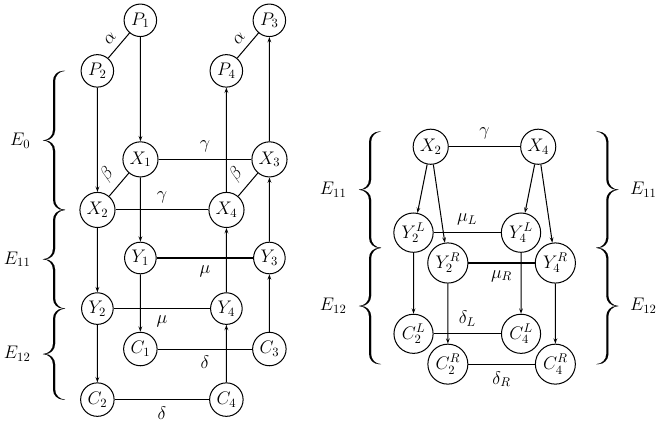
\includegraphics[width=0.6\columnwidth]{images/retracing_boomerang.png}
    \caption{The retracing boomerang attack.}
    \label{fig:retr-boomerang}
\end{figure}

\subsection{The Shifting Retracing Attack}

Assuming that \(pq_1q_2^Lq_2^R \gg 2^{-n/2}\), we can use the standard boomerang
attack to build a distinguisher similar to \autoref{alg:boomerang-dist}. The
main idea of the shifting retracing attack is to add a \(\brak{b - 1}\)-bit
filtering in the middle of the attack procedure, which is to check if \(C_1^L
\oplus C_2^L = 0 \textrm{ or } \delta_L\). We discard all such pairs that do not
satisfy this relation. A \(\delta\)-shift is performed on the filtered
ciphertext pairs to get \(\brak{C_3, C_4}\).

The key idea of performing this filtering is that the two unordered pairs
\(\brak{C_1, C_3}\) and \(\brak{C_2, C_4}\) are \emph{equal}. Thus, if one of
these pairs satisfies the differential characteristic \(\delta_L
\xrightarrow{q_2^L} \mu_L\), the other pair will too, which increases the
probability of the boomerang distinguisher by \(\brak{q_2^L}^{-1}\).

Notice that any possible characteristic of \(\brak{E_{12}^L}\) has probability
at least \(2^{-b + 1}\), thus the overall probability of the distinguisher
increases by a factor of at most \(2^{b - 1}\). On the other hand, the filtering
only leaves \(2^{-b + 1}\) of the pairs, so there is no apparent gain. However,
this approach has the following advantages.

\begin{enumerate}
    \item \emph{Improving the signal to noise ratio.} Improving the probability
    by a factor of \(\brak{q_2^L}^{-1}\) improves the signal to noise ratio
    which ensures a higher fraction of the filtered pairs on average satisfy
    \(P_3 \oplus P_4 = \alpha\). Furthermore, the characteristic \(\beta
    \xrightarrow{p} \alpha\) for the pair \(\brak{X_3, X_4}\) can be replaced by
    a truncated differential characteristic \(\beta \xrightarrow{p^\prime}
    \alpha^\prime\) of higher probability.
    \item \emph{Reducing the data complexity.} Due to the filtering, the attack
    leaves fewer ciphertexts. This improves the complexity in cases where more
    decryption queries are made.
    \item \emph{Reducing the time complexity.} The filtering can also reduce the
    time complexity if it is dominated by the analysis of the plaintext pairs
    \(\brak{P_3, P_4}\).
\end{enumerate}

\subsection{The Mixing Retracing Attack}

In the shifting attack, the attacker forces equality between the unordered pairs
\(\brak{C_1^L, C_2^L}\) and \(\brak{C_3^L, C_4^L}\) using a \(\delta\)-shift.
Instead, in this type of attack, each ciphertext pair can be shifted by
\(\brak{C_1^L \oplus C_2^L, 0}\). The resulting ciphertexts are
\begin{align}
    C_3 &= \brak{C_3^L, C_3^R} = \brak{C_1^L \oplus \brak{C_1^L \oplus C_2^L}, C_1^R} = \brak{C_2^L, C_1^R}, \\
    C_4 &= \brak{C_4^L, C_4^R} = \brak{C_2^L \oplus \brak{C_1^L \oplus C_2^L}, C_2^R} = \brak{C_1^L, C_2^R}.
\end{align}
Again, the unordered pairs \(\brak{C_1^L, C_2^L}\) and \(\brak{C_3^L, C_4^L}\)
are equal. Further, we have \(C_1^R = C_3^R\) and \(C_2^R = C_4^R\), thus we
gain an additional factor of \(\brak{q_2^R}^{-2}\) for a total probability of
\(\brak{pq_1}^2q_2^L\). This mixing is also similar to the core step used in the
yoyo attack on AES.

\subsection{Comparison Between the Two Types of Retracing Attacks}

Although the mixing attack has a higher probability, the shifting attack is
better in various scenarios.
\begin{enumerate}
    \item \emph{Using structures.} In the shifting attack, the same
    \(\delta\)-shift is applied to all pairs of ciphertexts and the filtering is
    applied first to reduce the data complexity. This is not possible in the
    mixing attack since the shift is based on the ciphertext pair and nothing is
    discarded. 
    
    Typically, the basic boomerang attack is extended by adding a round at the
    top or bottom of the distinguisher. In such cases, the shifting attack can
    be used to obtain all ciphertexts, shift all of them by \(\delta\) and then
    decrypt all of them, simulatneously checking for the filter and condition
    between \(P_3\) and \(P_4\) using a hash table.
    
    \item \emph{Combination with \(E_{11}\).} In the mixing variant, the output
    difference of \(E_{12}^L\) is arbitrary and changes with each ciphertext
    pair. In most cases, there is no good combination between differential
    characteristics of \(\brak{E_{12}^L}^{-1}\) and \(\brak{E_{11}}^{-1}\) that
    can be used. For instance, in the yoyo attack, \(E_{11}\) is empty.

    \item \emph{Construction of `friend pairs'.} `Friend pairs' are pairs that
    are attached to other pairs which satisfy a common property. There are many
    more `friend pairs' that can be constructed in the shifting variant, making
    it advantageous.
\end{enumerate}

\section{Retracing Boomerang Attack on Five Round AES}

The retracing boomerang attack is based on the yoyo attack, which is described
first.

\subsection{The Yoyo Attack on Five Round AES}

The yoyo attack decomposes 5-round AES as \(E = E_{12} \circ E_{11} \circ E_0\)
where \(E_0\) consists of the first 2.5 rounds, \(E_{11}\) is the first MC
operation of round 2 and \(E_{12}\) consists of rounds 3 and 4. 

For \(E_0\) in the forward direction, the adversary uses a trucated differential
characteristic whose input difference is zero in three inverse shifted columns
and whose output difference is zero in a single shifted column. The probability
of this characteristic is \(4 \cdot 2^{-8} = 2^{-6}\), since it holds iff the
output difference of the active column in round 0 is zero in at least one byte.

For \(E_{12}\) in the backward direction, notice that 1.5 rounds of AES can be
taken as four 32-bit super S-boxes. For each ciphertext pair \(\brak{C_1,
C_2}\), the adversary modifies it into its mixture \(\brak{C_3, C_4}\) with
respect to the super S-boxes and asks for their decryption. Due to the mixture
construction, the four inputs to the S-boxes have an XOR of zero, therefore
\(X_1 \oplus X_2 \oplus X_3 \oplus X_4 = 0\) as well since MC is linear.
Therefore, with probability \(2^{-6}\), we have \(X_3 \oplus X_4 = 0\) in a
shifted column. Subsequently, \(Z_3 \oplus Z_4 = 0\) in an inverse shifted
column, which corresponds to one of the four quartets \(\brak{0,5,10,15},
\brak{1,4,11,14}, \brak{2,5,8,13}, \brak{3,6,9,12}\). This can be used to set up
an attack on bytes \(\brak{0,5,10,15}\) of the subkey \(k_{-1}\). To get more
information about \(k_{-1}\), friend pairs of \(\brak{Z_3, Z_4}\) are used.

The yoyo attack has data complexity about \(2^9\) and overall time complexity is
\(2^{40}\). A careful analysis of round 0 can reduce the complexity down to
\(2^{31}\) encryptions. However, there is a better improvement that can be made
using a meet in the middle (MITM) attack on bytes 0, 5, 10 and 15 of \(k_{-1}\).
Denote the intermediate value of byte \(m\) before the \(MC\) operation of round
0 during encryption as \(W_m\), and consider WLOG \(l = 0\). Then, the input to
round 1 satisfies
\begin{equation}
    Z_0 = 02_x \cdot W_0 \oplus 03_x \cdot W_1 \oplus 01_x \cdot W_2 \oplus 01_x \cdot W_3.
    \label{eq:mitm}
\end{equation} 
In the MITM attack, the adversary guesses bytes 0, 5 of \(k_{-1}\) by computing
the values
\begin{equation}
    02_x \cdot \brak{\brak{W_3^j}_0 \oplus \brak{W_4^j}_0} \oplus 03_x \cdot \brak{\brak{W_3^j}_1 \oplus \brak{W_4^j}_1}
    \label{eq:mitm-0-5}
\end{equation}
for \(j = 1, 2, 3\), concatenating these values and storing them in a table for
each guess. Similarly, the adversary guesses the values for bytes 10, 15 of
\(k_{-1}\) and computes 
\begin{equation}
    01_x \cdot \brak{\brak{W_3^j}_2 \oplus \brak{W_4^j}_2} \oplus 01_x \cdot \brak{\brak{W_3^j}_3 \oplus \brak{W_4^j}_3}
    \label{eq:mitm-10-15}
\end{equation}
for \(j = 1, 2, 3\) and checks for a match in the table, which is equivalent to
the condition \(\brak{Z_3^j}_0 = \brak{Z_4^j}_0\) for \(j = 1, 2, 3\). This
24-bit filtering leaves \(2^8\) candidates for bytes 0, 5, 10, 15 of \(k_{-1}\).
These can be checked by using the conditions \(\brak{Z_3^4}_0 = \brak{Z_4^4}_0\)
and \(\brak{Z_1}_0 = \brak{Z_2}_0\).

Although the data complexity looks like \(2^{16}\), the \emph{dissection
technique} can be used to maintain the memory at \(2^9\). The time complexity is
now reduced to \(2^6 \cdot 4 \cdot 2^{16} = 2^{24}\) operations, which is
roughly equivalent to less than \(2^{23}\) encryptions.

\subsection{Improved Attack on Five Round AES}

The MITM attack can be improved to a time complexity of \(2^{16.5}\) at the
expense of incereasing the data complexity to \(2^{15}\). The main idea is to
reduce the number of possible key values to \(2^8\) instead of \(2^{16}\) as
described earlier. This is done in multiple steps.

\subsubsection{Specific Choice of Plaintexts}

To reduce the number of possible values of \(k_{-1, \cbrak{0, 5}}\), we choose
plaintexts with non-zero difference only in bytes 0 and 5. For such pairs, the
condition \(\brak{Z_1}_0 = \brak{Z_2}_0\) becomes
\begin{equation}
    02_x \cdot \brak{\brak{W_1}_0 \oplus \brak{W_2}_0} \oplus 03_x \cdot \brak{\brak{W_1}_1 \oplus \brak{W_2}_1}.
    \label{eq:mitm-simple}
\end{equation}
This equation is now an 8-bit filtering and leaves only \(2^8\) candidates for
\(k_{-1, \cbrak{0, 5}}\).

To detect the right key bytes efficiently, an even more specific choice of
plaintexts is used. We choose plaintexts \(\brak{P_1, P_2}\) satisfying
\(\brak{P_1}_5 \oplus \brak{P_2}_5 = 01_x\). Additionally, the row of the
difference distribution table (DDT) of the AES S-box corresponding to the input
difference \(01_x\) is computed and stored it in memory, where each output
difference is stored along with the value(s) that lead to it. Thus, for each
pair \(\brak{P_1, P_2}\) and for each guess of \(k_{-1, 0}\), we can use
\eqref{eq:mitm-simple} to compute the output difference of the SB operation in
byte 5. Since the input difference in this byte is \(01_x\), a lookup can be
used to find the inputs that can lead to this difference and retrieve possible
values of \(k_{-1, 5}\) that correspond to the guessed \(k_{-1, 0}\). This gives
us \(2^8\) values of \(k_{-1, \cbrak{0, 5}}\) in about \(2^8\) simple operations
per pair.

\subsubsection{Eliminating Key Bytes Using Friend Pairs}

To reduce the number of possible values of \(k_{-1, \cbrak{10, 15}}\), the
boomerang process is used to return multiple friend pairs \(\brak{P_3^j,
P_4^j}\). In particular, we choose one such pair for which
\begin{equation}
    \brak{P_3^j}_{10} \oplus \brak{P_4^j}_{10} = 0 \quad \textrm{or} \quad \brak{P_3^j}_{15} \oplus \brak{P_4^j}_{15} = 0.
    \label{eq:mitm-check}
\end{equation}
Assume WLOG that equality holds in byte 10. Then, \eqref{eq:mitm-10-15} depends
only on \(k_{-1, 15}\) and thus has only \(2^8\) possible values. This procedure
requires \(2^9\) simple operations and leaves \(2^8\) suggestions for \(k_{-1,
\cbrak{0, 5, 15}}\) since this is an additional 8-bit filtering. Finally,
another friend pair can be taken and a similar MITM procedure followed to obtain
the unique value of \(k_{-1, \cbrak{0, 5, 10, 15}}\) by isolating the
contribution of \(k_{-1, 10}\).

Therefore, the time complexity of this MITM attack is reduced to about \(2^8\)
operations for each pair \(\brak{P_1, P_2}\) and for each value of \(l\). This
totals to about \(2^{16}\) operations. For each pair, we require \(2^7\) friend
pairs to find one that satisfies \eqref{eq:mitm-check} with high probability.
Hence, the total data complexity is increased to about \(2^{15}\).

\subsubsection{Attack Algortihm}

The improved attack algorithm is described below.

\begin{enumerate}
    \item \textbf{Precomputation:} Compute the row of the DDT of the AES S-box
    that corresponds to input difference \(01_x\), along with the actual values
    that lead to this difference.
    \item \textbf{Online Phase:} Take 64 pairs \(\brak{P_1, P_2}\) of plaintexts
    such that in each pair, \(\brak{P_1}_5 = 00_x\) and \(\brak{P_2}_5 = 01_x\),
    \(\brak{P_1}_0 \ne \brak{P_2}_0\) and all other corresponding bytes are
    equal.
    \item For each plaintext pair, create \(2^7\) `friend pairs' \(\brak{P_1^j,
    P_2^j}\) such that for each \(j\) we have \(P_1^j \oplus P_2^j = P_1 \oplus
    P_2\) and \(\brak{P_1^j}_{\cbrak{0, 5, 10, 15}} = \brak{P_1}_{\cbrak{0, 5,
    10, 15}}\).
    \item For each plaintext pair \(\brak{P_1, P_2}\) and for each \(l \in
    \cbrak{0, 1, 2, 3}\), do the following. (Here, \(l = 0\) is taken for
    convenience.)
    \begin{enumerate}
        \item For each guess of \(k_{-1, 0}\), partially encrypt \(\brak{P_1,
        P_2}\) through \(SB\) in byte 0 of round 0 to find the output
        difference. Then, assuming \(\brak{P_1, P_2}\) satisfies \(E_0\), that
        is, \(\brak{Z_1}_0 = \brak{Z_2}_0\), use \eqref{eq:mitm-simple} to find
        the output difference of the \(SB\) operation in byte 5 of round 0. Use
        the precomputed DDT to deduce inputs to the \(SB\) operation in byte 5
        of round 0. Consequently, deduce the value of \(k_{-1, 5}\) for this
        guess of \(k_{-1, 0}\). Store all \(2^8\) possible values of \(k_{-1,
        \cbrak{0, 5}}\) in a table.
        \item Ask for the encryption of \(\brak{P_1, P_2}\) and of its friend
        pairs \(\brak{P_1^j, P_2^j}\). For each ciphertext pair \(\brak{C_1,
        C_2}\) or \(\brak{C_1^j, C_2^j}\), replace it by its mixture
        counterparts to obtain \(\brak{C_3, C_4}\) or \(\brak{C_3^j, C_4^j}\).
        Ask for the decryption of these pairs, and let them be \(\brak{P_3,
        P_4}\) and \(\brak{P_3^j, P_4^j}\).
        \item Find a \(j\) for which \eqref{eq:mitm-check} is satisfied.
        \item Perform an MITM attack on column 0 of round 0 using the
        corresponding pair \(\brak{P_3^j, P_4^j}\) to obtain \(2^8\) possible
        values of \(k_{-1, \cbrak{0, 5, 15}}\).
        \item Perform another MITM attack on column 0 of round 0 using two
        plaintext pairs \(\brak{P_3^{j^\prime}, P_4^{j^\prime}}\). For each
        guess of \(k_{-1, 10}\), compute the contribution of byte 2 to
        \eqref{eq:mitm-simple} and check for a collision. This gives a possible
        value for \(k_{-1, \cbrak{0, 5, 10, 15}}\). If a contradiction is
        reached, move to the next value of \(l\). If a contradiction is reached
        for all values of \(l\), discard the pair \(\brak{P_1, P_2}\) and move
        on to the next pair.
    \end{enumerate}
    \item Using a pair \(\brak{P_1, P_2}\) for which no contradiction occurred
    along with its `friend pairs', perform MITM attacks on columns 1, 2 and 3 of
    round 0 using the fact that \(Z_3 \oplus Z_4\) equals 0 in the \(l\)-th
    inverse shifted column to recover the entire subkey \(k_{-1}\). 
\end{enumerate}

\subsubsection{Attack Analysis}
The attack succeeds if the data contains a pair that satisfies the truncated
differential characteristic of \(E_0\) and for one of the `friend pairs' of that
pair, the corresponding plaintext pair \(\brak{P_3^j, P_4^j}\) has zero
difference in either byte 10 or 15. With 64 plaintext pairs and 128 `friend
pairs' per plaintext pair, each of these events occur with probability \(1 -
e^{-1} \approx 0.63\) giving us a probability of success of \(0.63^2 = 0.4\).
Increasing the number of initial pairs and friend pairs per initial pair will
boost the success probability.

Another way of boosting the succees probability is to find other ways to cancel
terms in \eqref{eq:mitm-10-15}. For instance, if there exist \(j, j^\prime\)
such that \(\cbrak{\brak{P_3^j}_{10}, \brak{P_4^j}_{10}} =
\cbrak{\brak{P_3^{j^\prime}}_{10}, \brak{P_4^{j^\prime}}_{10}}\), we can take
the XOR of \eqref{eq:mitm-10-15} to cancel the effect of \(k_{-1, 10}\), thus
increasing the success probability even when there is no pair that satisfies
\eqref{eq:mitm-check}.

The data complexity of the above attack is \(2 \cdot 2^6 \cdot 2^7 = 2^{14}\)
chosen plaintexts and \(2^{14}\) adaptively chosen ciphertexts. One can use
structures to reduce the data complexity to slightly above \(2^{14}\) adaptively
chosen ciphertexts and plaintexts, but this also slightly reduces the success
probability due to additional dependencies between analyzed pairs. 

The memory complexity of the attack remains at \(2^9\) 128-bit memory cells,
like the yoyo attack.

The time complexity is dominated by several MITM attacks that take \(2^{16}\)
operations each. Considering one AES operation to be equivalent to 80 S-box
lookups and adding it to the number of queries gives us a total of \(2^{16.5}\)
encryptions.

\section{Improved Attack on Five Round AES with a Secret S-box}

The retracing boomerang technique can be used to devise an attack on five round
AES with a secret S-box. This attack recovers the secret key without fully
recovering the secret S-box (the S-box is recovered upto an affine
transformation in \(GF\brak{2^8}\)). The idea is to start with exploiting the
fact that with probability \(2^{-6}\), the pair \(\brak{Z_3, Z_4}\) has zero
difference in an inverse shifted column. This observation does not depend on the
specific structure of \(MC\) and \(SB\) operations, hence it can be applied to
key-dependent variants as well.

\subsection{Partial Recovery of the S-box}

Assume WLOG that the retracing boomerang produces zero difference in byte 0 of
state \(Z\), that is, \(\brak{Z_3}_0 \oplus \brak{Z_4}_0 = 0\). \eqref{eq:mitm}
can be rewritten as
\begin{align}
    0 &= \brak{Z_3}_0 \oplus \brak{Z_4}_0 \\
    &= 02_x \cdot \brak{\brak{W_3}_0 \oplus \brak{W_4}_0} \oplus 03_x \cdot \brak{\brak{W_3}_1 \oplus \brak{W_4}_1} \oplus 01_x \cdot \brak{\brak{W_3}_2 \oplus \brak{W_4}_2} \oplus 01_x \cdot \brak{\brak{W_3}_3 \oplus \brak{W_4}_3}.
    \label{eq:lin-secret}
\end{align}
Note that \(\brak{W_3}_j = SB\brak{P_3 \oplus k_{-1, j^\prime}}\) for \(j = 0,
1, 2, 3\) where \(j^\prime = SR^{-1}\brak{j}\). Therefore, if we define \(4
\cdot 256 = 1024\) variables \(x_{m,j} = SB\brak{m \oplus k_{-1, j^\prime}}\)
for \(m \in \bF_q\) and \(j = 0, 1, 2, 3\), then each plaintext pair \(P_1,
P_2\) which satisfies \eqref{eq:lin-secret} provides a linear equation in the
variables \(x_{m,j}\). To obtain many pairs, we attach about \(2^{10}\) `friend
pairs' to each of the \(2^6\) original pairs \(\brak{P_1, P_2}\). For each
original pair along with its `friend pairs', we perform the mixing retracing
boomerang process to obtain a linear equation in the variables \(x_{m, j}\). A
few more friend pairs are taken for extra filtering of the original pairs.

Since we are working with differences in \eqref{eq:lin-secret}, we can recover
the S-box with an invertible linear transformation over \(GF\brak{2^8}\). In
other words, we can only obtain functions \(S_0, S_1, S_2, S_3\) such that
\begin{equation}
    S_j\brak{x} = L_0\brak{SB\brak{x \oplus k_{-1, j^\prime}}},
\end{equation}
for some unknown linear transformation \(L_0\). Similar linear transformations
\(L_t\) will be obtained for column \(t\).

\subsection{Recovering the Secret Key}

The secret key \(k_{-1}\) can be recovered despite not knowing the S-box in two
steps.

First, for each \(j^\prime\), we can recover \(\bar{k_{j^\prime}} = k_{-1, 0}
\oplus k_{-1, {j^\prime}}\) as \(\bar{k_{j^\prime}}\) is the unique value of
\(c\) such that \(S_j\brak{x} = S_0\brak{x \oplus c}\) for all \(x\). Similarly,
we can recover each inverse shifted column of \(k_{-1}\) up to \(2^8\) possible
values. This reduces the total number of candidates for \(k_{-1}\) to
\(2^{32}\).

Second, the differences \(k_{-1, 0} \oplus k_{-1, j}\) for \(j = 1, 2, 3\) can
be found by taking several quartets of values \(\brak{x_0, x_1, x_2, x_3}\) such
that \(\bigoplus_{i=0}^3S_0\brak{x_i} = 0\). These quartets eliminate the effect
of the difference between the linear transformations \(L_0\) and \(L_j\) by
finding the unique value of \(c_j\) such that \(\bigoplus_{i=0}^3 S_j\brak{c_j
\oplus x} = 0\). Thus, in about \(2^{12}\) operations, we can determine the
entire secret key \(k_{-1}\) upto the value of \(k_{-1, 0}\). These \(2^8\)
possibilities can be exhaustively searched.

\subsection{Attack Analysis}
The data complexity of this attack is \(2 \cdot 2^6 \cdot 2^{10} = 2^{17}\)
chosen plaintexts and \(2^{17}\) adaptively chosen ciphertexts. Using
structures, the amount of chosen plaintexts can be reduced to \(2^{14}\), thus
the overall data complexity is less than \(2^{17.5}\) chosen plaintexts and
adaptively chosen ciphertexts.

The time complexity is dominated by solving a system of 1034 equations in 1024
variables for each of the \(2^6\) pairs \(\brak{P_1, P_2}\). Using an efficient
algorithm such as the Method of the Four Russians, each solution takes about
\(2^{27}\) simple operations or approximately \(2^{21}\) encryptions. Thus, the
overall time complexity is \(2^{29}\).

The memory complexity is dominated by the memory required for solving the
equations, which is about \(2^{17}\) 128-bit blocks.

\subsection{Improvement Using a Distinguisher Before the Attack}

The equation solving step has to be applied \(2^8\) times since we do not know
if a pair satisfies the boomerang property. To obtain this information in
advance, we can use the five-round yoyo distinguisher. In this variant, the time
complexity is dominated by the complexity of the yoyo distinguisher, which is
\(2^{25.8}\). The memory complexity is still \(2^{17}\).

\section{The Retracing Rectange Attack and Mixture Differentials}

A drawback of the retracing boomerang attack is that it uses the stronger
adaptively chosen plaintext and ciphertext model. However, the amplified
boomerang attack uses only the chosen plaintext model of attack. We first
explore this attack before introducing the retracing variant.

\subsection{The Amplified Boomerang Attack}

In this version of the boomerang attack, the adversary considers \emph{pairs of
pairs} of plaintexts \(\brak{\brak{P_1, P_2}, \brak{P_3, P_4}}\) such that \(P_1
\oplus P_2 = P_3 \oplus P_4 = \alpha\). For each such pair, the adversary then
checks whether the corresponding quartet of ciphertexts \(\brak{\brak{C_1, C_2},
\brak{C_3, C_4}}\) satisfy \(C_1 \oplus C_2 = C_3 \oplus C_4 = \delta\).

The analysis behind this distinguisher is that the overall probability of the
boomerang is \(p^2q^2\), thus if \(pq \gg 2^{-n/2}\), then a distinguisher can
be created using \(4 \cdot 2^{n/2}\brak{pq}^{-1}\) chosen plaintexts. The time
complexity of this attack is \(\cO\brak{2^{n/2}\brak{pq}^{-1}}\) using hash
tables.

\subsection{The Retracing Rectangle Attack}

Translating a retracing boomerang attack to a retracing rectangle attack follows
the same idea as translating a (classical) boomerang attack to a rectangle
attack. We start with decomposing \(E = E_1 \circ E_{02} \circ E_{01}\), where
\(E_{01}\) divides the state into two parts of \(b\) and \(n - b\) bits.
Further, suppose that there exists differential characteristics \(\alpha_L
\xrightarrow{p_1^L} \mu_L\) for \(E_{01}^L\), \(\alpha_R \xrightarrow{p_1^R}
\mu_R\) for \(E_{01}^R\), \(\mu \xrightarrow{p_2} \beta\) for \(E_{02}\) and
\(\gamma \xrightarrow{q} \delta\) for \(E_1\). This is illustrated in
\autoref{fig:retr-rectangle}.

\begin{figure}
    \centering
    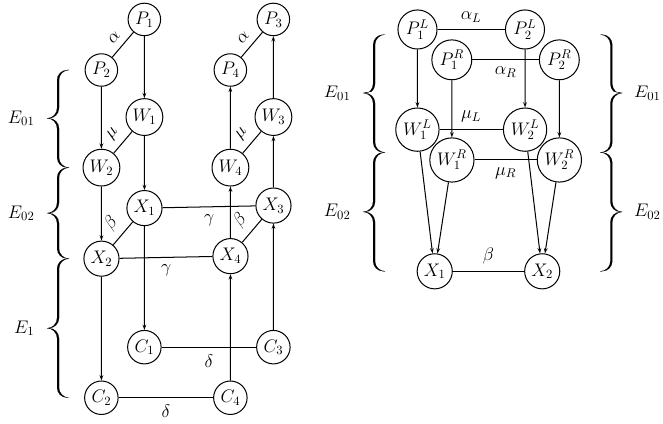
\includegraphics[width=0.6\columnwidth]{images/retracing_rectangle.png}
    \caption{The retracing rectangle attack.}
    \label{fig:retr-rectangle}
\end{figure}

A distinguisher can be built assuming \(p_1^Lp_1^Rp_2q \gg 2^{-n/2}\) as before.
However, in the retracing rectangle attack, we consider plaintext quartets that
satisfy
\begin{equation}
    \brak{P_1 \oplus P_2 = \alpha} \land \brak{P_3 \oplus P_4 = \alpha} \land \brak{P_1^L \oplus P_3^L = 0 \textrm{ or } \alpha_L}.
    \label{eq:retr-rect-cond}
\end{equation}
As a result of \eqref{eq:retr-rect-cond}, \(\cbrak{P_1^L, P_2^L} = \cbrak{P_3^L,
P_4^L}\). If one of them satisfies the differential characteristic of
\(E_{10}^L\), then so does the other. This improves the probability of the
distinguisher by a factor of \(\brak{p_1^L}^{-1}\).

Unlike the shifting retracing boomerang attack, there is no need to filter data
to obtain an improvement. Additionally, the signal to noise ratio is improved.
Usually, the adversary starts with a structure \(\cS\) of plaintext pairs with
input difference \(\alpha\). Instead of checking all \(\binom{\abs{\cS}}{2}\)
pairs, a hash table is used to check all quartets in \(\cO\brak{\abs{\cS}}\)
time.

\subsection{Mixing Variant and Relation to Mixture Differentials}

Similar to the mixing retracing boomerang attack, the adversary can force,
\(\cbrak{P_1^L, P_2^L} = \cbrak{P_3^L, P_4^L}\) by choosing \(P_3 = \brak{P_2^L,
P_1^R}\) and \(P_4 = \brak{P_1^L, P_2^R}\). As this choice forces
\(\cbrak{P_1^R, P_2^R} = \cbrak{P_3^R, P_4^R}\), the probability of the
rectangle distinguisher is increased by a factor of \(\brak{p_1^Lp_1^R}^{-1}\).

\end{document}
